\documentclass[conference]{IEEEtran}
\usepackage{booktabs}
\usepackage{graphicx}
\usepackage{amsmath}
\usepackage{amssymb}
\usepackage{array}
\usepackage{url}
\usepackage[hidelinks]{hyperref}
\usepackage{etoolbox}

\newcommand{\feat}[1]{\texttt{#1}}

% Reclaim the inter-float glue so the eight-page limit holds without cutting content.
\setlength{\textfloatsep}{6pt plus 2pt minus 2pt}
\setlength{\dbltextfloatsep}{6pt plus 2pt minus 2pt}
\setlength{\floatsep}{4pt plus 1pt minus 1pt}
\setlength{\dblfloatsep}{4pt plus 1pt minus 1pt}
\setlength{\abovecaptionskip}{3pt}
\setlength{\belowcaptionskip}{0pt}

\patchcmd{\thebibliography}{\footnotesize}{\scriptsize}{}{}
\setlength{\columnsep}{0.16in}

\begin{document}

\title{NATRIX: An Auditable Feature-Admission and Promotion Protocol for Inline HTTP Attack Detection}

\author{
\IEEEauthorblockN{Ahire Nameet Sudam}
\IEEEauthorblockA{Department of Computer Engineering\\
Sardar Patel Institute of Technology, Mumbai 400058, India}
\and
\IEEEauthorblockN{D. D. Ambawade}
\IEEEauthorblockA{Department of Computer Engineering\\
Sardar Patel Institute of Technology, Mumbai 400058, India}
}

\maketitle

\begin{abstract}
Web application firewalls must decide inline, yet the evidence behind their feature sets, promotion rules, and latency budgets is rarely auditable. NATRIX is a role-based HTTP attack-detection architecture that separates a five-role synchronous decision path from four asynchronous governance roles; this paper evaluates its feature-admission gate and promotion protocol, not the full orchestration. The contribution is an auditable feature-admission procedure with a measured cost gate, a model-checked promotion protocol, and an evaluation showing that WAF detector rankings invert between deployment-like and endpoint-disjoint splits. The detector contract is request-level: method, path, query, body, and user agent. A three-gate mechanism combines provenance and safety constraints, a frozen four-condition statistical drop rule, and a measured extraction-cost budget; applied to 34,593 deduplicated CSIC 2010 requests, it reduces a 22-dimensional contract to 20 dimensions with a written evidence row for every decision, and rejects all 12 statistically accepted candidates because their measured cost exceeds the budget. The promotion protocol is model-checked in TLA+, mutation-tested (6/6 guards killed), and verified on 81,484 exact-rational trust-decay cases. The central evaluation finding is a protocol inversion: under a deployment-like split the lexical full-request baseline beats NATRIX on all three corpora, while under an endpoint-disjoint split the full-request baseline collapses on CSIC and the payload-only view wins; on SR-BH the payload view collapses and the path carries the signal. The ranking is therefore protocol- and view-dependent, and a single-protocol headline is not evidence of payload detection. v4 is not claimed to be more accurate or meaningfully faster; its value is that every feature's presence or removal is justified by recorded evidence. Inline p95 is 3.78\,ms over 9,700 requests. No live-traffic claim is made.
\end{abstract}

\begin{IEEEkeywords}
web application firewall, role-based security architecture, HTTP attack detection, feature selection, formal verification, TLA+, evaluation protocol, trust.
\end{IEEEkeywords}

\section{Introduction}
A web application firewall (WAF) sits on the request path and must return a verdict in milliseconds. Modern deployments combine signature rules such as the OWASP Core Rule Set (CRS) with learned detectors, yet three questions are usually unanswered. Why is each feature in the detector contract? What evidence permits a candidate rule to become active policy? Does the reported accuracy survive a protocol that removes endpoint identity? A trial-and-error feature set cannot be audited, a hit-counter promotion path can entrench a false positive, and a headline from a random split can be an endpoint prior rather than a payload signal.

This paper presents NATRIX as an answer to those questions and evaluates it as an \emph{auditable feature-admission and promotion protocol}, not as a state-of-the-art classifier. The architecture separates five synchronous roles that produce a per-request verdict from four asynchronous governance roles that change future policy. Only the gate and CPPP are evaluated here; the role decomposition is a design framework, not a detection gain. The contract is request-level---method, path, query, body, and user agent---and a payload-only contract is a different object, evaluated here as a diagnostic view.

The contribution is an auditable feature-admission procedure with a measured cost gate, a model-checked promotion protocol, and an evaluation showing that WAF detector rankings invert between deployment-like and endpoint-disjoint splits. (i) A protocol inversion: under P1 the lexical full-request baseline is stronger than NATRIX on all three corpora, but under P2 it collapses on CSIC while the payload view stays at 96.03\%, and on SR-BH the payload view collapses while the path carries the signal. (ii) A three-gate admission mechanism: Gate A checks provenance, observability, determinism, and a frozen safety list; Gate B applies a frozen four-condition statistical rule (C1--C4); Gate C applies a measured extraction-cost budget. On CSIC 2010 it reduces a 22-dimensional contract to 20 dimensions, and a 24-candidate screen accepts 12 statistically while admitting none because the accepted block costs 1.71\,ms p95 against a 0.15\,ms budget. (iii) CPPP, a promotion protocol with quorum, canary, trust, and audit guards; a \feat{SeedTrust} action decouples trust from votes so the quorum invariant is falsifiable, and the protocol is model-checked, mutation-tested, and verified on exact-rational trust decay. (iv) An evaluation protocol that reports every in-distribution result under P1 and P2, with lexical views, a generic control, cross-fitted stackers, a nested threshold check, a frozen CRS replay, and a dilution test. None of the individual components is new; the contribution is the combination and the evidence standard.

The inversion is the organising result: a P1-only paper would declare the full-request lexical model best on every corpus, a P2-only paper would declare NATRIX best on none. We do not claim that NATRIX is the best detector, that it generalises across populations, that the proxy enforces CPPP, or that any result is validated on live traffic.

\begin{quote}
\small
\textbf{Contributions.} An auditable feature-admission procedure with a measured cost gate; a model-checked promotion protocol; a two-protocol evaluation that shows detector rankings invert between P1 and P2; and a reproducibility artifact with the evidence row for every admission and rejection.\\[2pt]
\textbf{Non-contributions.} Not a new classifier; not state of the art; no live-traffic or shadow-mode validation; no adaptive-adversary evaluation; and CPPP is not implemented in the shipped proxy.
\end{quote}

\section{Related Work}
Signature WAFs such as ModSecurity with CRS remain the operational baseline~\cite{ristic2010modsecurity,owasp_crs}; their rules are interpretable, but the operating point is a configuration choice. Learned HTTP detection ranges from n-gram and classical models to transformer representations~\cite{kruegel2003anomaly,robertson2006behavior,garcia2009anomaly,torrano2010anomaly,sureda2022new,luo2026wadbert}. WADBERT reports F1 99.64 on CSIC and 99.59 on SR-BH~\cite{luo2026wadbert}, but released no code or model and its protocol is not reproduced here; we cite it with a caveat.

Sommer and Paxson argued that machine-learning intrusion detection is often evaluated in ways that do not transfer to deployment~\cite{sommer2010outside}. Arp et al. documented data snooping and inappropriate baselines~\cite{arp2022dos}; Pendlebury et al. showed that test-set transitivity can inflate Android malware detection~\cite{pendlebury2019tesseract}; drift explains why a fixed boundary degrades~\cite{gama2014survey}. P1/P2 follows this line: the endpoint view tests whether a headline is an endpoint prior, and the payload view tests whether the signal survives without the path.

Feature selection is grouped into filter, wrapper, and embedded methods~\cite{guyon2003introduction}. Permutation importance~\cite{breiman2001random} and SHAP~\cite{lundberg2017unified} are descriptive tools, not decision rules; Rudin argues that post-hoc explanation is not a substitute for an interpretable model~\cite{rudin2019stop}. Pre-registration guards against adapting the analysis to the data~\cite{nosek2018preregistration}. Our C1--C4 thresholds and cost budget are frozen before the v4 outcome is inspected. CPPP is closer to a finite-state security protocol: TLA+ and TLC~\cite{lamport2002specifying,clarke2009model} check the specification, and zero-trust principles~\cite{nist2020zero} motivate separating evidence producers from the policy owner.

\textbf{Positioning.} Prior feature-selection work reports a final set and its accuracy, but not a measured admission cost, a promotion protocol, or a protocol-inversion check. Prior WAF evaluations usually report one split, and prior role-based architectures specify authority without model-checking promotion. None of the components is new: filter and wrapper selection, permutation importance, extraction-cost budgets, TLA+ checking, and endpoint-disjoint splits all predate this paper. The contribution is the combination and the evidence standard: every decision has a recorded row, the cost gate is measured on the worst case, promotion is model-checked, and the ranking is reported under both protocols.

\section{Architecture and Threat Model}
\subsection{Roles and the Synchronous/Asynchronous Split}
Fig.~\ref{fig:arch} shows the architecture. Telemetry Ingestion parses the request and computes the active contract; Zero-Trust Verifier checks identity and context and may veto independently; Threat Intelligence supplies signature evidence; ML Engine runs the gate and typing model and has no promotion authority; Remediation Orchestrator fuses evidence and emits the only inline block. Four roles are asynchronous: Risk Scoring aggregates session risk, Adaptive Memory stores incident summaries and drift indicators, Policy Agent owns the candidate lifecycle and is the only role allowed to promote or retire, and Containment executes post-decision side effects. Governance stays off the latency path, and the authority graph is acyclic: evidence producers cannot change policy, and the policy owner cannot fabricate evidence.

\begin{figure*}[t]
\centering
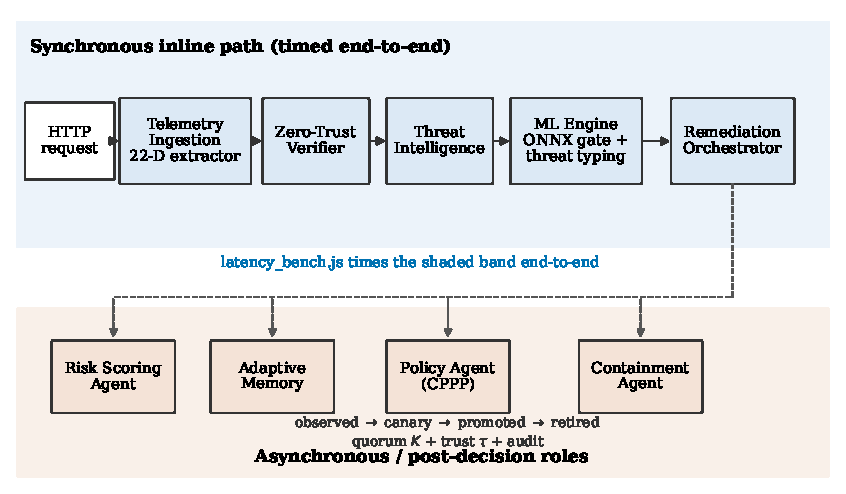
\includegraphics[width=0.54\textwidth]{../figures/architecture.pdf}
\caption{NATRIX architecture. The synchronous path contains five roles and produces the per-request verdict. The asynchronous band contains four governance roles. Only the Policy Agent may promote a candidate, and promotion requires quorum, canary evidence, trust, and an audit record.}
\label{fig:arch}
\end{figure*}

\subsection{Request Path, Verdict, and Contract Scope}
The inline path is HTTP request $\rightarrow$ Telemetry Ingestion $\rightarrow$ Zero-Trust Verifier $\rightarrow$ Threat Intelligence $\rightarrow$ ML Engine $\rightarrow$ Orchestrator. The verdict is allow, block, or challenge; policy is a function of the evidence tuple, not a hard-coded threshold on the model alone. The headline accuracy numbers are gate numbers; the orchestration logic is specified and unit-tested but is not the object of the accuracy claim.

The contract uses method, path, query, body, and user agent; it excludes response bodies, logs, DNS, and external reputation. The path is included deliberately: a WAF sees it, and endpoint structure is real evidence. The paper therefore says \emph{request contract}, not \emph{payload contract}. The lexical baseline's payload view excludes the path and is a diagnostic, not a description of NATRIX.

\subsection{Threat Model and Shipped Runtime}
The adversary controls method, path, query, headers, body, encoding, and user agent, and may attempt SQL injection, XSS, traversal, command injection, XXE, Log4Shell-style lookups, and obfuscation. We assume agent processes, model artifacts, and the audit log are not compromised, and that votes carry authenticated agent identity. CPPP addresses unauthorised promotion by one agent and promotion without canary or quorum; it does not address Byzantine collusion, Sybil identities, model poisoning, or supply-chain compromise. The evaluation is not an adaptive-evasion study.

The current proxy implements the inline path and a simplified promotion path: a new signature is inserted with \feat{hitCount = 1}, the next observation increments the count, and the candidate becomes active when \feat{hitCount >= 2} or the source contains \feat{PCAP} or \feat{Dataset}. There is no canary, independent quorum, trust value, or automatic decay---exactly the transition CPPP forbids. The formal results are about the specified protocol and its reference implementation, not the shipped proxy; replacing the shortcut is the deployment step.

\section{CPPP and Trust Decay}
\subsection{Lifecycle, SeedTrust, and Invariants}
CPPP is a finite-state protocol for candidate rules and models. A candidate is observed, canary, promoted, retired, or rejected. Allowed transitions are observed$\rightarrow$canary, canary$\rightarrow$promoted or rejected, promoted$\rightarrow$retired, and observed$\rightarrow$rejected by policy. There is no observed$\rightarrow$promoted transition, no path in which one agent both supplies the only vote and promotes, and no promotion without an audit record. Quorum counts independent agent identities, not messages, so repeated votes from one agent do not count twice. The canary is the only source of live promotion evidence and cannot be skipped; the Policy Agent cannot satisfy the quorum alone.

An earlier model coupled trust to votes: an agent gained trust by voting, and quorum was counted over agents already above the floor. The invariant was close to true by construction, and a mutant that removed the quorum guard could survive. The revision adds a \feat{SeedTrust} action that sets trust independently of any vote. Votes are recorded separately, and the promotion guard checks both. TLC checks seven safety invariants: \feat{TypeOK}; \feat{NoPromotionWithoutCanary}; \feat{NoPromotionWithoutQuorum}; \feat{NoPromotionWithoutTrust}; \feat{ActiveImpliesAudited}; \feat{RetiredNotActive}; and \feat{NoDirectPromotion}. These are safety, not liveness, properties.

\subsection{Trust Decay}
Trust is a scalar in $[0,1]$. Without evidence it decays as $T(t)=T_0e^{-\lambda t}$; positive evidence raises trust towards 1 with gain $\alpha\in(0,1]$: $E(T)=T+\alpha(1-T)$. The implementation uses an exact rational discrete model. One scheduler tick applies decay with factor $\rho\in(0,1)$, then reinforcement:
\begin{equation}
\operatorname{tick}(T)=\rho T+\alpha(1-\rho T).
\end{equation}
Under stationary evidence the fixed point and closed form are
\begin{equation}
T^\ast=\frac{\alpha}{1-(1-\alpha)\rho},\qquad
T_n=T^\ast+(T_0-T^\ast)\bigl((1-\alpha)\rho\bigr)^n.
\end{equation}
The contraction factor $(1-\alpha)\rho$ is strictly below 1, so the iteration converges geometrically. A promoted rule whose trust falls below the floor $\tau$ is retired atomically on the tick that would cross it.

\subsection{Verification and Sensitivity}
TLC checks the one-rule and two-rule configurations (459 and 114,901 states; depth 11 and 18) with no error, and breadth-first enumeration of the executable reference to depth 9 covers 13,278 states and 62,263 transitions with no invariant violation. The mutation test removes one guard at a time; all six mutants are killed, including \feat{no\_quorum}, \feat{no\_canary}, \feat{no\_trust}, \feat{no\_audit}, \feat{direct\_promote}, and \feat{retired\_active}. Trust decay is checked on 81,484 exact-rational cases with zero violations, and nine symbolic identities are proved with SymPy. A sidecar over 700 audit records verified the hash chain and all six runtime invariants. Promotion and retirement cost 3.63 and 3.33\,ms p95 without fsync (34.18 and 34.44\,ms with fsync); validation is 42.70\,ms p95 and should be batched or moved off the critical path.

For five agents with no compromise, raising $K$ from 2 to 4 reduces the promotion probability at weak honest validation ($p=0.2$) from 0.263 to 0.007; with two compromised agents, $K=2$ is already saturated. A slow decay ($\rho=0.95$) gives a half-life of 14 ticks; a fast decay ($\rho=0.50$) gives 1 tick. The paper reports the trade-off rather than an optimum.

\section{Three-Gate Feature Admission}
\subsection{Feature Origin}
v1 (10 features) was the first prototype, drawn from common WAF indicators: request length, Shannon entropy, character-class ratios, token count, SQL/XSS/traversal keyword scores, and a scanner user-agent flag. v2 (16) added six threat-typing features: command-injection patterns, encoding ratio, null-byte flag, duplicate-parameter count, HTML tag density, and method risk. v3 (22) added six lexical gate features: suspicious extensions, quote and angle counts, double escapes, and maximum parameter-value ratio and length. Seven safety features come from rules the runtime already enforced as policy. Every feature is computable from request fields the inline proxy already has; none needs a response body, logs, DNS, or external reputation. The v3 block and candidate pool were shaped by error inspection of gate misses, but v1-to-v3 growth was iterative, not frozen in advance; admission came afterwards to audit the result. The paper reports that sequence, not a one-pass design. Formula, source, and safety status of every feature are in \texttt{tables/feature\_contract.csv} in the repository.

\subsection{Contract Versions and Gate A}
The runtime has four contracts. v1 is a 10-dimensional prototype set; v2 a 16-dimensional threat-typing set; v3 the 22-dimensional request contract used by the binary gate; v4 the 20-dimensional contract produced by admission. The versions share extraction code and differ only in the feature mask; the ONNX export preserves the input order expected by the service. The 22 v3 features cover shape, lexical counts and maxima, evasion signals, signature scores, structural counts, and method risk.

Gate A requires a feature computable from fields the inline proxy already has, deterministic, bounded in cost, and independent of response bodies, logs, DNS, and external reputation. It must not be on the frozen safety list. That list is a design exception: seven features are retained because the runtime uses them as direct policy signals (\feat{sql\_keyword\_score}, \feat{xss\_keyword\_score}, \feat{path\_traversal\_score}, \feat{command\_injection\_score}, \feat{null\_byte\_score}, \feat{request\_method\_risk}, \feat{user\_agent\_anomaly}). Removing one from the model contract would not remove the policy rule; it would only mislead the audit.

\subsection{Gate B: The Frozen Four-Condition Rule}
A feature is dropped only if all four conditions hold. \textbf{C1 (univariate):} the Benjamini--Hochberg adjusted $p$-value is at least 0.05 and the absolute Cliff's delta below 0.10, or the feature is near-constant (zero fraction at least 0.99 in both classes). \textbf{C2 (importance):} permutation importance is in the bottom quartile and its 95\% bootstrap interval contains zero. \textbf{C3 (ablation):} leave-one-feature-out ablation shows no degradation larger than the practical-equivalence margin (accuracy change at most 0.2 points, FPR change at most 0.10 points, interval excluding a harmful drop). \textbf{C4 (safety):} the feature is not on the safety list. The conjunction is conservative: a feature weak univariately but important in the model is retained, one important but redundant in ablation is retained, and a statistically droppable safety signal is retained.

\subsection{Gate C, Decision Rule, and Outcome}
Gate C requires added p95 extraction cost on the 8\,KiB worst case to be at most 0.15\,ms; a feature that fails Gate C is not admitted even if Gate B accepts it:
\begin{equation}
\operatorname{admit}(f)=\mathrm{Gate\,A}(f)\land\mathrm{Gate\,B}(f)\land\mathrm{Gate\,C}(f).
\end{equation}
A feature is \emph{dropped} only if Gate A passes, Gate B fails, and it is not on the safety list. A feature that passes Gate B but fails Gate C is \emph{not admitted}, not statistically useless. The distinction is recorded in the evidence table; there is no post-hoc rescue.

Applied to the 22-dimensional v3 contract on CSIC 2010, the rule drops exactly two features: \feat{param\_pollution\_count} and \feat{html\_tag\_density}. Both are exactly zero in both classes, so C1 holds by the near-constant clause, and their importance and ablation are null. The retained contract is 20-dimensional. This is a CSIC-only result: both features are constant on this corpus, so the evidence cannot show whether they carry signal elsewhere; they may. The cross-corpus audit is descriptive and does not re-run selection. Table~\ref{tab:evidence} gives the four-condition row for every feature. \feat{token\_count} is the conservative case: its permutation importance is $-0.00054$ with a 95\% interval of $[-0.00082,-0.00026]$, strictly below zero, so C2 fails and it is retained. \feat{special\_char\_ratio} is the opposite anomaly: strongly associated univariately and seventh in permutation importance, yet leave-one-out ablation shows that removing it \emph{improves} accuracy by 1.52 points (95\% CI [1.37, 1.68]) and lowers FPR by 0.24 points. C3 catches a harmful drop, not a beneficial removal, so the frozen rule retains it; a post-hoc designer would drop it and report the gain. The 1.52 points bound what the rule leaves on the table.

\begin{table}[t]
\caption{Gate B evidence for all 22 v3 features on CSIC 2010. Y means the drop condition is met; a feature is dropped only when C1--C4 are all Y. $^{\dagger}$Safety-retained policy signal. The rule drops two constant features and retains \feat{token\_count} because C2 requires an interval containing zero, not a negative one.}
\label{tab:evidence}
\centering
\scriptsize
\setlength{\tabcolsep}{3pt}
\begin{tabular}{@{}lccccc@{}}
\toprule
Feature & C1 & C2 & C3 & C4 & Decision\\
\midrule
\feat{param\_pollution\_count} & Y & Y & Y & Y & drop\\
\feat{html\_tag\_density} & Y & Y & Y & Y & drop\\
\midrule
\feat{sql\_keyword\_score}$^{\dagger}$ & N & N & Y & N & retain\\
\feat{request\_method\_risk}$^{\dagger}$ & N & N & N & N & retain\\
\feat{xss\_keyword\_score}$^{\dagger}$ & N & Y & Y & N & retain\\
\feat{path\_traversal\_score}$^{\dagger}$ & Y & Y & Y & N & retain\\
\feat{user\_agent\_anomaly}$^{\dagger}$ & Y & Y & Y & N & retain\\
\feat{command\_injection\_score}$^{\dagger}$ & Y & Y & Y & N & retain\\
\feat{null\_byte\_score}$^{\dagger}$ & Y & Y & Y & N & retain\\
\midrule
\feat{uppercase\_ratio} & N & N & N & Y & retain\\
\feat{hex\_encoding\_ratio} & N & N & N & Y & retain\\
\feat{digit\_ratio} & N & N & N & Y & retain\\
\feat{payload\_length} & N & N & N & Y & retain\\
\feat{max\_value\_special\_ratio} & N & N & N & Y & retain\\
\feat{shannon\_entropy} & N & N & N & Y & retain\\
\feat{special\_char\_ratio} & N & N & Y & Y & retain\\
\feat{max\_value\_length} & N & N & N & Y & retain\\
\feat{double\_escape\_count} & N & N & N & Y & retain\\
\feat{quote\_count} & N & N & Y & Y & retain\\
\feat{suspicious\_extension\_flag} & N & N & Y & Y & retain\\
\feat{angle\_count} & N & Y & Y & Y & retain\\
\feat{token\_count} & Y & N & Y & Y & retain\\
\bottomrule
\end{tabular}
\end{table}

v4 is statistically equivalent to v3 on CSIC: both reach 95.55\% at the cross-fitted point, v3 has 1.94\% FPR and v4 1.96\%, the paired difference is $-0.01$ points $[-0.07,+0.06]$, and McNemar $p=0.8624$; the nested policy gives 94.67/1.26 and 94.59/1.24. The dropped features are constant zero on every CSIC request, so removing them cannot change a tree partition. v4 is not claimed to be more accurate or meaningfully faster; its value is that every feature's presence or removal is justified by recorded evidence.

The same mechanism screened 24 frozen candidates from the literature, runtime capability, and error analysis. Twelve pass the statistical screen (mean delta F1 above its standard error and positive in four of five folds). None is admitted: the accepted block costs 1.71\,ms p95 against the 0.15\,ms budget, and the full pass costs 2.33\,ms. Five accepted candidates (\feat{backslash\_count}, \feat{brace\_count}, \feat{nonascii\_ratio}, \feat{ldap\_filter\_score}, \feat{crlf\_sequence\_count}) are constant on CSIC, so their identical $+0.046$-point gain is an RNG artefact; the rest need a second body pass or full Unicode normalisation. The paper answers ``why is this feature here?'' for all 22 and ``why not?'' for all 24; that negative decision is designed, not a failure to find a better model.

\textbf{How to add a feature.} The procedure is fixed before the candidate is scored.
\begin{enumerate}
\item Implement it in the Node and Python extractors with identical logic.
\item Gate A: available request fields only; deterministic, bounded cost.
\item Reject if constant on the corpus or $|\text{Spearman}| \ge 0.95$ with an existing feature.
\item Add it to the 20-feature core; run the same five folds; accept only if the mean F1 gain exceeds its standard error and is positive in four of five folds.
\item Gate C: measure the accepted block's p95 cost on the 8\,KiB worst case against the 0.15\,ms budget.
\item Write the evidence row and decision before looking at final test results.
\end{enumerate}

\section{Evaluation Protocol}
\label{sec:protocol}
Four labelled HTTP corpora are used. CSIC 2010~\cite{csic2010dataset} is the primary benchmark: 97,065 raw requests deduplicate to 34,593 unique requests (18,640 clean, 15,953 attack) on (method, path, query, body, user agent), with no label conflicts. ECML/PKDD 2007~\cite{raissi2007web} contains 50,116 requests (35,006 clean, 15,110 attack) with seven attack classes. SR-BH 2020~\cite{srbh2020dataset} parses to 907,815 rows; deduplication removes 485,237 duplicates and 524 conflicts, leaving 422,054 unique requests (122,546 clean, 299,508 attack) and 338,640 endpoint groups. OpenAppSec WCP 2024~\cite{openappsec2024} provides 137,820 legitimate requests and 73,924 malicious payloads; every malicious row has path \texttt{/}, so a random split leaks the endpoint. WCP is diagnostic only.

\textbf{P1 (deployment-like).} Stratified five-fold over unique requests. No identical request crosses the split, but the same endpoint may appear in training and test. This matches WAF operation, where the endpoint is known and the question is whether a request to it is malicious. \textbf{P2 (endpoint-disjoint).} Stratified group five-fold. A group is (method, normalised path, query keys, body keys) and is assigned wholly to one fold. P2 is the generalisation bound, never the headline. It is not path-free: the path string remains a feature; P2 removes the endpoint's identity as a memorisable training item. P2 folds are built once per corpus and reused by every score-based detector, so the comparison is paired.

The primary learner is the shipped gate: a Random Forest with 200 trees, unlimited depth, \feat{min\_samples\_leaf=1}, \feat{max\_features=None}, no class weighting, and \feat{random\_state=42}, pinned to the deployed artifact and not tuned on test folds. The lexical baseline is a hashed character 2--4 gram representation ($2^{18}$ dimensions) with an L2-regularised logistic-loss SGD classifier at $\alpha=10^{-5}$, 30 epochs, and averaging; it has endpoint, payload, and full views. An independent character-level CNN (32-dimensional byte embedding, two convolutions, five epochs) is trained on the same folds and calibrated identically. The generic control is a 17-feature LightGBM over request-shape descriptors with no security keywords. CRS is the official \texttt{owasp/modsecurity-crs} 4.25.2 nginx image at PL1--PL3, anomaly threshold 5, request-body inspection on, response-body off.

All score-based detectors use leave-one-fold-out thresholds at FPR $\le 2\%$, the deployment policy; a fully nested inner-five-fold policy is a stricter check. Confidence intervals are percentile bootstrap with 2,000 resamples~\cite{efron1993introduction}; paired comparisons use McNemar's test~\cite{mcnemar1947note} and a paired bootstrap, read descriptively~\cite{demsar2006statistical}. The feature audit uses Benjamini--Hochberg correction across the 22 tests~\cite{benjamini1995controlling}. The latency path is the real Node proxy, HTTP \texttt{/predict}, ONNX inference, threat typing, and verdict; it excludes synchronous SQLite writes, disk logging, and containment. The input is 10,000 real requests (5,000 CSIC, 3,000 ECML, 2,000 WCP); after 300 warm-up, 9,700 are measured with zero failures.

\section{Results}
\subsection{Matched Operating Points}
Table~\ref{tab:detectors} reports the cross-fitted FPR $\le 2\%$ point under both protocols. Under P1, NATRIX reaches 95.55/1.93 on CSIC, 91.96/1.67 on ECML, and 90.79/1.96 on the SR-BH 20k sample. The lexical full-request baseline is stronger on every corpus at the same policy: 96.57/1.96, 93.93/0.43, and 95.41/1.98. The lexical payload view is also stronger on CSIC and ECML but collapses on SR-BH (36.20\% accuracy, 10.91\% recall). CRS PL1 is not competitive.

\begin{table*}[t]
\caption{Matched operating points at the cross-fitted FPR $\le 2\%$ policy. P1 is deployment-like; P2 is endpoint-disjoint. CRS is a frozen PL1 replay and is not tuned to 2\%. SR-BH rows use the shared 20k sample. Values are percentages.}
\label{tab:detectors}
\centering
\scriptsize
\setlength{\tabcolsep}{4pt}
\begin{tabular}{@{}llrrrrrr@{}}
\toprule
 & & \multicolumn{3}{c}{P1 (deployment-like)} & \multicolumn{3}{c}{P2 (endpoint-disjoint)}\\
\cmidrule(lr){3-5}\cmidrule(lr){6-8}
Corpus & Detector & Acc & FPR & Rec & Acc & FPR & Rec\\
\midrule
CSIC & NATRIX & 95.55 & 1.93 & 92.60 & 78.85 & 6.50 & 61.73\\
CSIC & Lex-full & 96.57 & 1.96 & 94.84 & 69.53 & 21.57 & 59.13\\
CSIC & Lex-payload & 96.90 & 1.88 & 95.47 & 96.03 & 2.43 & 94.24\\
CSIC & CRS PL1 & 66.24 & 0.03 & 26.84 & -- & -- & --\\
ECML & NATRIX & 91.96 & 1.67 & 77.19 & 91.60 & 1.75 & 76.21\\
ECML & Lex-full & 93.93 & 0.43 & 80.85 & 93.76 & 0.51 & 80.47\\
ECML & Lex-payload & 92.66 & 0.54 & 76.90 & 92.70 & 0.44 & 76.81\\
SR-BH & NATRIX 20k & 90.79 & 1.96 & 87.82 & 90.62 & 1.88 & 87.56\\
SR-BH & Lex-full & 95.41 & 1.98 & 94.34 & 94.75 & 2.01 & 93.43\\
SR-BH & Lex-payload & 36.20 & 2.00 & 10.91 & 36.27 & 1.88 & 10.97\\
SR-BH & CRS PL1 & 44.29 & 25.80 & 32.00 & -- & -- & --\\
\bottomrule
\end{tabular}
\end{table*}

Under P2, NATRIX falls to 78.85/6.50 on CSIC, lexical full to 69.53/21.57, while lexical payload stays at 96.03/2.43 with 94.24\% recall. The full-request lexical model used endpoint identity; on unseen endpoints that prior generates false positives. On SR-BH, lexical full stays at 94.75/2.01 and lexical payload collapses to 36.27/1.88 with 10.97\% recall: the path carries the signal and generalises to unseen groups. An independent char-CNN reproduces the inversion (CSIC P2 full 85.45/21.63, payload 96.03/1.57; SR-BH P1 full 95.34/2.36, payload 36.05/1.95). The collapse is a property of the protocol and view, not the learner. Neither protocol alone is universal; Fig.~\ref{fig:protocol} plots the matched points.

\begin{figure*}[t]
\centering
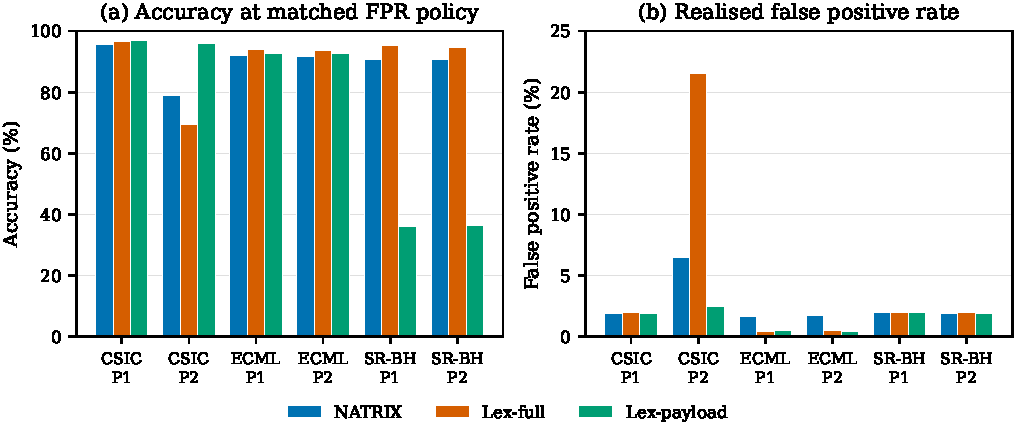
\includegraphics[width=0.68\textwidth]{../figures/revision_protocol_sensitivity.pdf}
\caption{Matched operating points for NATRIX, lexical full-request, and lexical payload under P1 and P2. Panel (a) is accuracy and panel (b) is realised FPR. The CSIC P2 panel shows the endpoint-disjoint collapse of the full-request lexical model; the SR-BH P2 panel shows the opposite payload collapse.}
\label{fig:protocol}
\end{figure*}

\subsection{View Ablation}
\label{sec:views}
Table~\ref{tab:views} reports five views. On SR-BH P1, full reaches 90.79/1.96 with 87.82\% recall; removing path-derived features drops recall to 12.74\%, while a path-only model retains 85.53\%. Query-only and body-only models reach 11.10\% and 9.58\% recall. P2 gives 90.62/1.88, 12.49\%, and 85.31\%. Path morphology, not endpoint memorisation, carries the SR-BH signal, so SR-BH is not payload evidence.

On CSIC P2 the pattern inverts. Full reaches 78.85/6.50 with 61.73\% recall; no-path reaches 75.07/4.26 with 50.92\%, only 3.78 points below full at a lower FPR. A path-only model has 74.64\% recall but flags 99.92\% of clean requests, so accuracy collapses to 34.47\%. The path adds recall at a false-positive cost: on CSIC P2 lexical payload beats NATRIX full, while on SR-BH P2 NATRIX full beats lexical payload.

\begin{table}[t]
\caption{View ablation on the 22-D contract at the cross-fitted FPR $\le 2\%$ policy. Values are percentages.}
\label{tab:views}
\centering
\footnotesize
\setlength{\tabcolsep}{4pt}
\begin{tabular}{@{}llrrr@{}}
\toprule
Protocol & View & Acc & FPR & Rec\\
\midrule
SR-BH P1 & full & 90.79 & 1.96 & 87.82\\
SR-BH P1 & no-path & 37.52 & 1.93 & 12.74\\
SR-BH P1 & path-only & 89.16 & 1.98 & 85.53\\
SR-BH P2 & full & 90.62 & 1.88 & 87.56\\
SR-BH P2 & no-path & 37.29 & 2.08 & 12.49\\
SR-BH P2 & path-only & 89.05 & 1.83 & 85.31\\
CSIC P2 & full & 78.85 & 6.50 & 61.73\\
CSIC P2 & no-path & 75.07 & 4.26 & 50.92\\
CSIC P2 & path-only & 34.47 & 99.92 & 74.64\\
\bottomrule
\end{tabular}
\end{table}

\subsection{CRS Paranoia Levels}
\label{sec:crs}
The same 34,593 CSIC requests were replayed through CRS at PL1--PL3; the full table is in the repository (\texttt{tables/crs\_paranoia.md}). At PL1, CRS reaches 66.24\% accuracy at 0.03\% FPR with 26.84\% recall: it blocks 4,281 of 15,953 attacks and only 6 of 18,640 clean requests. PL2 gives 63.82/16.07/40.35 (F1 0.51) and PL3 51.91/71.21/78.92 (F1 0.60); p95 latency is 318, 1,730, and 1,877\,ms. The paranoia level is a recall/FPR dial: PL2 exceeds the 2\% budget eightfold and PL3 flags seven in ten legitimate requests. It is not a substitute for a learned payload model.

\subsection{SR-BH Scale}
The SR-BH full-versus-20k gap is a sample-size effect. The full corpus reaches 95.70/1.95 with 94.74\% recall; the 20k sample reaches 90.79/1.96 with 87.82\% recall: a 4.91-point accuracy and 6.92-point recall gap at nearly the same FPR. Attack prevalence (70.96\% vs 70.97\%) and the SQL-injection share (63.77\% vs 63.30\%) are matched, so the prior is not the explanation. The nested curve is monotonic: 10k 87.86, 20k 90.31, 50k 93.43, 100k 94.09, 200k 95.00, full 95.70. Under P2 the 20k sample reaches 90.62/1.88 and the full corpus 94.01/2.77, so scale does not remove the endpoint-disjoint penalty. No full-scale ranking is claimed because the lexical baseline is replayed only on the sample.

\subsection{Dilution and the v3-D Variant}
The bounded mutation suite applies the full mutation set to all 15,953 CSIC attacks. v3 reaches 92.60\% clean recall; under mutation it falls to 82.47\% ($-10.13$ points) and 2,639 attacks that v3 originally blocked are evaded (17.86\%). v3-D adds nine per-parameter and per-path maxima to stop an ignored appended parameter from diluting an aggregate ratio. It reaches 96.79\% accuracy at 2.08\% FPR with 95.46\% clean recall; mutated recall is 85.51\% ($-9.95$ points) and 2,222 attacks are evaded. On the targeted subset (14,350 attacks with a query or body), v3 falls from 91.83\% to 58.51\% ($-33.32$ points, 5,197 evaded) and v3-D from 94.99\% to 66.55\% ($-28.44$ points, 4,387 evaded). The targeted loss is 4.88 points smaller, but a 28-point loss remains: the fix is partial.

\subsection{Controls, Fusion, Latency, and Parity}
The generic 17-feature control is weaker than NATRIX at the same budget everywhere, including CSIC P2 (67.65/30.80 with 65.84\% recall) and SR-BH P2 (71.96/2.00 with 61.30\% recall). The NATRIX+lexical stacker improves on the lexical base on CSIC P1 (98.45/1.24 with 98.08\% recall; nested 98.24/1.32 with 97.72\% recall), on ECML P2 (94.02/0.35 vs 93.76/0.51), and on SR-BH P2 full by 1.46 points. It does not improve on CSIC P2 full ($-1.98$ points) or CSIC P2 payload ($-0.14$), because the full stack inherits both base scores' endpoint failure. The SR-BH P2 payload ``gain'' (+55.18 points over lexical payload) is the NATRIX path signal re-entering the stack, not a payload-fusion effect. Gate-plus-CRS OR fusion is redundant on CSIC ($+14$ attacks for $+6$ false positives, $p=0.115$) and over budget elsewhere (ECML 1.67\%$\to$21.19\%, SR-BH 1.96\%$\to$27.16\%, WCP 0.11\%$\to$6.71\% FPR). These are negative results for naive score fusion; the full control and stacker table is in the repository (\texttt{tables/control\_stack\_compact.md}).

Over 9,700 measured requests, the p50 is 2.86\,ms, the p95 is 3.78\,ms, and the p99 is 5.69\,ms; the worst request is 32.68\,ms. The HTTP hop dominates: its p95 is 3.61\,ms, extraction 0.20\,ms, and ONNX scoring 0.004\,ms. Per-corpus p95 is 3.86\,ms (CSIC), 3.54\,ms (ECML), and 3.85\,ms (WCP); the 8\,KiB adversarial worst case is 6.68\,ms. A p95 is not a hard bound. ONNX parity over 79,593 records gives a maximum absolute probability difference of $1.79\times10^{-7}$ for the gate and $1.26\times10^{-7}$ for the typing model; all label disagreements are exact ties.

A same-machine microbenchmark isolates the 22-D to 20-D difference on the same 10,000 frozen inputs (300 warm-up, median of three passes). Python extraction p95 is 0.54\,ms for v3 and 0.49\,ms for a benchmark-only 20-D path that skips the dropped features ($\Delta=-0.05$\,ms); p50 is 0.234\,ms for both. Single-threaded ONNX p95 is 0.46\,ms for the shipped 22-D gate and 0.47\,ms for a 20-D forest trained only for timing ($\Delta=+0.02$\,ms). The 20-D model is not an accuracy artifact, and the differences are within run-to-run noise at p95; v4 is not claimed to be meaningfully faster.

\section{Discussion and Limitations}
\label{sec:discussion}
The evidence supports five claims, none state-of-the-art: the three-gate mechanism is a reusable decision procedure (22$\rightarrow$20 with every row justified, 0/24 admitted on cost); inline p95 is 3.78\,ms and the HTTP hop dominates; CPPP is model-checked, mutation-tested, and implemented; the comparison protocol is itself a contribution, since NATRIX is competitive under P1 but does not beat the lexical baseline and P2 changes the ranking by corpus; and the dilution fix is a partial improvement.

It does not support universal generalisation: ECML misses the 95\% target, P2 fails on CSIC, and the 20k sample understates full SR-BH by 4.91 points. Transfer is severe (AUC 0.435 and 0.486, below chance; ten features reverse direction). It does not show that NATRIX is best, that v4 improves accuracy, that the detector is adversarially robust, that gate+CRS fusion helps at 2\%, that the proxy enforces CPPP, or that the results hold on live traffic.

\textbf{Limitations.} CSIC and ECML are old; SR-BH is attack-dominant; WCP is site-clustered with all malicious paths \texttt{/}; none is a probability sample. Labels use different ontologies. P1 inflates performance; P2 is the bound and fails on CSIC. The nested policy misses 95\% by 0.33--0.41 points; the cross-fitted policy is not fully nested. The forest is pinned; secondary learners and the generic control are fixed references. TLC covers three agents and two rules; BFS is bounded at depth 9; Byzantine faults, Sybil identities, poisoning, and supply chain are out of scope. Latency is a single-workstation component measurement excluding writes, logging, and containment. The mutation study is bounded, not adaptive. CRS is a frozen configuration; the lexical baseline is not a reproduction of a named system. Baselines are replayed only on 20k SR-BH, so no full-scale ranking is claimed. All evidence is offline.

\textbf{Implications.} Preserve the inline/async split; calibrate per deployment (0.5 gives 2.07/7.56/1.50\% FPR on CSIC/SR-BH/ECML); treat feature direction as non-portable; fix transport before the forest for a hard bound; require a complementary learned second agent; and make endpoint-only and payload-only baselines mandatory in WAF papers.

\section{Conclusion}
The contribution is an auditable feature-admission procedure with a measured cost gate, a model-checked promotion protocol, and an evaluation showing that WAF detector rankings invert between deployment-like and endpoint-disjoint splits. The positive results are concrete: a 20-dimensional contract with a written justification for every decision; a 24-candidate screen that admits none because cost exceeds budget; a model-checked promotion protocol with six of six mutants killed and 81,484 exact-rational decay cases; and an inline p95 of 3.78\,ms with a p99 of 5.69\,ms. The negative results are equally concrete: a lexical full-request baseline is stronger under P1 on every corpus, and a char-CNN is comparable on CSIC; P2 fails on CSIC; SR-BH is carried by path morphology; transfer AUCs are below chance; CRS fusion is negative at 2\%; v4 is not claimed to be more accurate or meaningfully faster; and the targeted dilution attack still removes 28.44 points with v3-D. The architecture and the evidence standard are reusable even though the detector is neither universal nor state of the art. Future work includes a shadow-mode canary, adaptive adversarial evaluation, and a dilution-invariant maximum-over-parameters contract. A reproducibility package with the feature extractor, experiment scripts, ONNX artifacts, formal models, and manuscript build is at \url{https://github.com/NameetAhire/natrix-auditable}.

\bibliographystyle{IEEEtran}
\bibliography{refs}

\end{document}
